\documentclass[10pt,a4paper]{article}
\usepackage[left=2cm,right=2cm,top=2cm,bottom=2cm]{geometry}
\usepackage[dvipsnames]{xcolor}
\usepackage[fleqn]{mathtools}
\usepackage{booktabs}
\usepackage{amsmath}
\usepackage{latexsym}
\usepackage{graphicx}
\usepackage{nccmath}
\usepackage{multicol}
\usepackage{listings}
\usepackage{tasks}
\usepackage{color}
\usepackage{float}
\usepackage{lipsum}

\definecolor{colorIPN}{rgb}{0.5, 0.0,0.13}
\definecolor{colorESCOM}{rgb}{0.0, 0.5,1.0}
\graphicspath{ {imagenes/} }

\begin{document}
%#########################################################
\begin{titlepage}
	\centering
	{ \huge \bfseries \color{colorIPN}{Instituto Politécnico Nacional} \par}
	{ \Large \bfseries  \color{colorESCOM}{Escuela Superior de Cómputo} \par }
	\vspace{1cm}
	{\huge\Large \color{colorIPN}{Tecnologías para Desarrollo de Aplicaciones Web}.\par}
	\vspace{1.5cm}
	{\huge\Large  \color{colorESCOM}{Avance del Proyecto: Aplicación Web para reporte de ventas de una tienda de conveniencia}\par}
		\vspace{2cm}
	{\Large\itshape \color{colorIPN}{Profesor: M. en C. José Asunción Enríquez Zárate}\par} \hfill \break
	{\Large\itshape \color{colorIPN}{Alumnos:}\par} \hfill \break
	{\Large\itshape \color{colorIPN}{Aguirre Cassandra}\par} \hfill \break
	{\Large\itshape \color{colorIPN}{Hernández Bryan}\par} \hfill \break
	{\Large\itshape \color{colorIPN}{Hurtado Morales Emiliano}\par} \hfill \break
	\vspace{1cm}
	{\Large\itshape \color{colorIPN}{Martínez Armando}\par} \hfill \break
	{\Large\itshape \color{colorIPN}{@alumno.ipn.mx}\par} \hfill \break
	{\Large\itshape \color{colorIPN}{@alumno.ipn.mx}\par} \hfill \break
	{\Large\itshape \color{colorIPN}{ehurtadom1700@alumno.ipn.mx}\par} \hfill \break
	{\Large\itshape \color{colorIPN}{@alumno.ipn.mx}\par} \hfill \break
	{\Large\itshape \color{colorIPN}{4CM3} \par}
	\vfill
	{\large \color{colorIPN}{\today}\par} 
	\vfill
\end{titlepage}

\renewcommand\lstlistingname{Quelltext} 

\lstset{ 
	language=Java,
	basicstyle=\small\sffamily,
	numbers=left,
	numberstyle=\tiny,
	frame=tb,
	tabsize=4,
	columns=fixed,
	showstringspaces=false,
	showtabs=false,
	keepspaces,
	commentstyle=\color{Violet},
	keywordstyle=\color{colorIPN} \bfseries,
	stringstyle=\color{colorESCOM}
}

\settasks{
	counter-format=(tsk[r]),
	label-width=4ex
}

\tableofcontents 
\pagebreak

\listoffigures
\pagebreak

%################################################
\section{\color{colorIPN}{Introducción}}
El reporte de ventas es un informe donde se recogen las actividades comerciales de una empresa. Su objetivo es evaluar el desempeño del departamento comercial, las estrategias de ventas y el trabajo de los representantes, para  identificar fallas y oportunidades de mejora en los procesos. 

La función principal del departamento comercial es atraer clientes, vender más y de forma más eficiente. El reporte de ventas es la herramienta que permite reunir y analizar el volumen de ventas de la empresa, determinar la efectividad de las acciones que realizas para generar ventas y evaluar la productividad de los agentes de ventas.

\subsection{ \color{colorESCOM}{Modelo E-R}}
Un modelo de entidad relación (modelo E-R) es el diseño de la estructura lógica de una base de datos, que luego se podrá implementar como una base de datos real. Los componentes principales del modelo E-R son un conjunto de entidades y de relaciones.

Un modelo de entidad relación describe cosas de interés interrelacionadas en un dominio específico de conocimiento. En ingeniería de software, el modelo E-R se utiliza generalmente para incorporar cosas que necesita recordar una empresa para efectuar los procesos empresariales.

\subsection{ \color{colorESCOM}{Modelo Relacional}}
Un modelo relacional consiste en representar datos por medio de tablas relacionadas cuyas filas se llaman tuplas y las columnas variables, conformando así una base de datos.

Existen una serie de términos formales que se corresponden con expresiones informales.

\begin{itemize}
	\item La relación, que es el término formal, tiene en la tabla su equivalente informal.
	\item La tupla no es más que un registro que se representa en las filas de la tabla y el atributo es una columna o campo.
	\item La cardinalidad se refiere al número de filas o registros y el grado es el número de columnas o campos.
	\item Por último, la clave primaria es un identificador único de cada caso.
\end{itemize}

\subsection{ \color{colorESCOM}{Diccionario de datos}}
Un diccionario de datos trata de documentar los metadatos más ligados a su almacenamiento en la base de datos. Es decir, incluye aspectos técnicos como el tipo de dato, formato, longitud, posibles valores que puede tomar e, incluso, transformaciones sufridas, sin olvidar la definición de cada campo. 

La documentación de estas transformaciones proporciona automáticamente el linaje del dato, entendido como la trazabilidad a lo largo de su ciclo de vida. Estos metadatos ayudan a los usuarios a entender los datos desde el punto de vista técnico para poder explotarlos adecuadamente. Por este motivo, cada base de datos debería contar con su diccionario de datos asociado. 
\pagebreak

%################################################
\section{\color{colorIPN}{Conceptos}}

\begin{itemize}
	\item  Entidad: Cualquier cosa en la empresa que se representará en la base de datos.
	\item  Atributo: Describe la propiedad de una entidad.
	\item  Atributo Clave: Identifica de forma exclusiva una entidad de un conjunto de entidades.
	\item Relación: Muestra cómo se relacionan las entidades entre sí.
	\item Cardinalidad: Especifica cuántas instancias de una entidad se relacionan con una instancia de otra entidad.
	\item Tabla: Herramienta de organización de información que se utiliza en bases de datos en la informática.
	
\end{itemize}

\pagebreak

%################################################
\section{\color{colorIPN}{Desarrollo}}
En este apartado, se presenta la estructura general de la base de datos del proyecto Registro de Ventas, mediante esta estructura se puede visualizar la manera en que se relacionan todos los elementos de la base de datos y los paquetes en los que se dividió la base de datos.

%################################################
\subsection{
	\textit{
		\color{colorESCOM}{Modelo E-R}
	}
}
El modelo de la base de datos, según la naturaleza de la información que cada una de ellas almacenará.

\begin{figure}[H]
	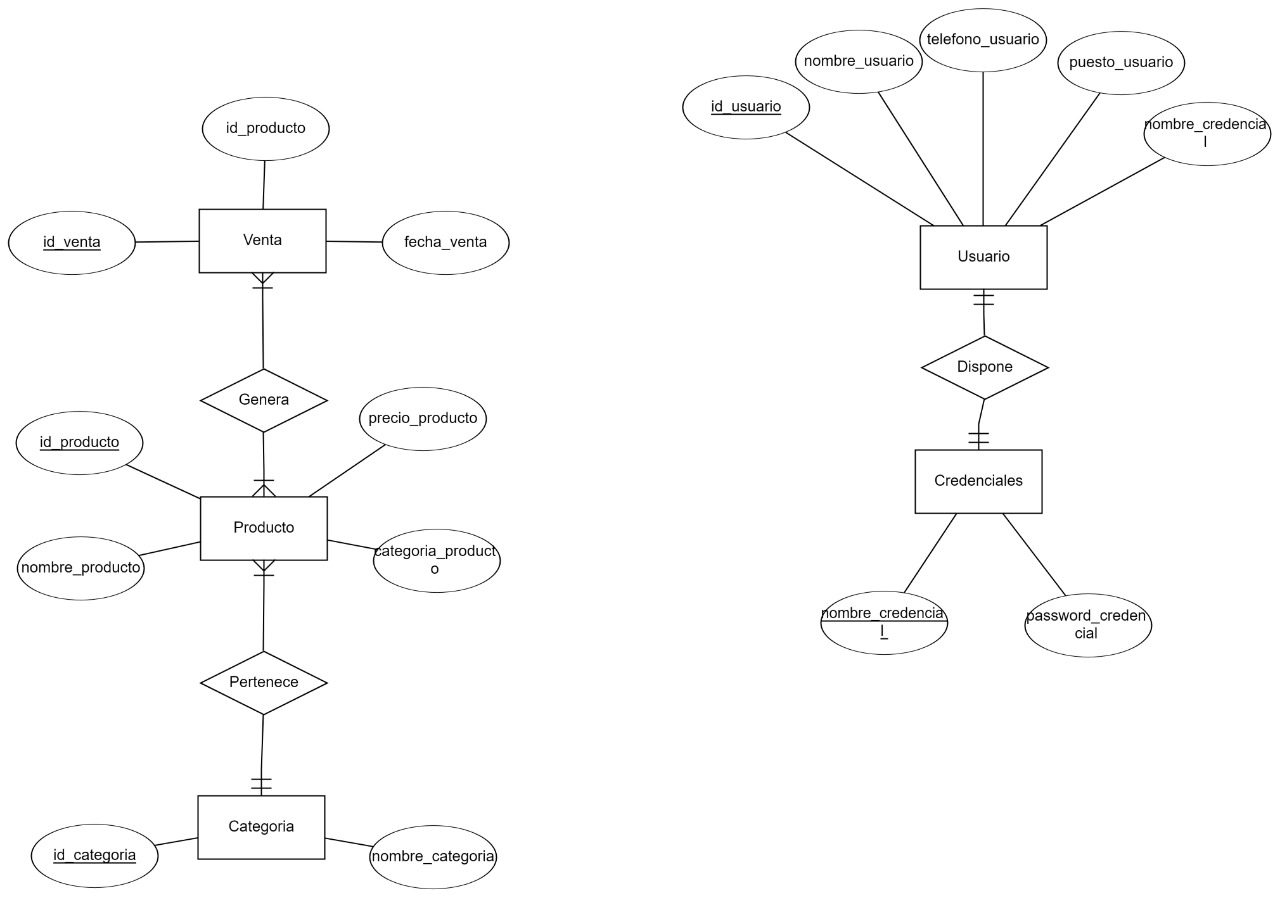
\includegraphics[scale=.45]{modeloER}
	\centering
	\caption{Diagrama E-R de base de datos}
	\label{img:modeloER}
\end{figure} 

\pagebreak

\subsection{
	\textit{
		\color{colorESCOM}{Modelo Relacional}
	}
}

La base de datos del sistema se ha segmentado en paquetes, según la naturaleza de la información
que cada una de ellas almacenará. Los paquetes se dividen en cinco segmentos que se muestran en el
diagrama de la figura 2 y se mencionan a continuación:
	
	\begin{figure}[H]
		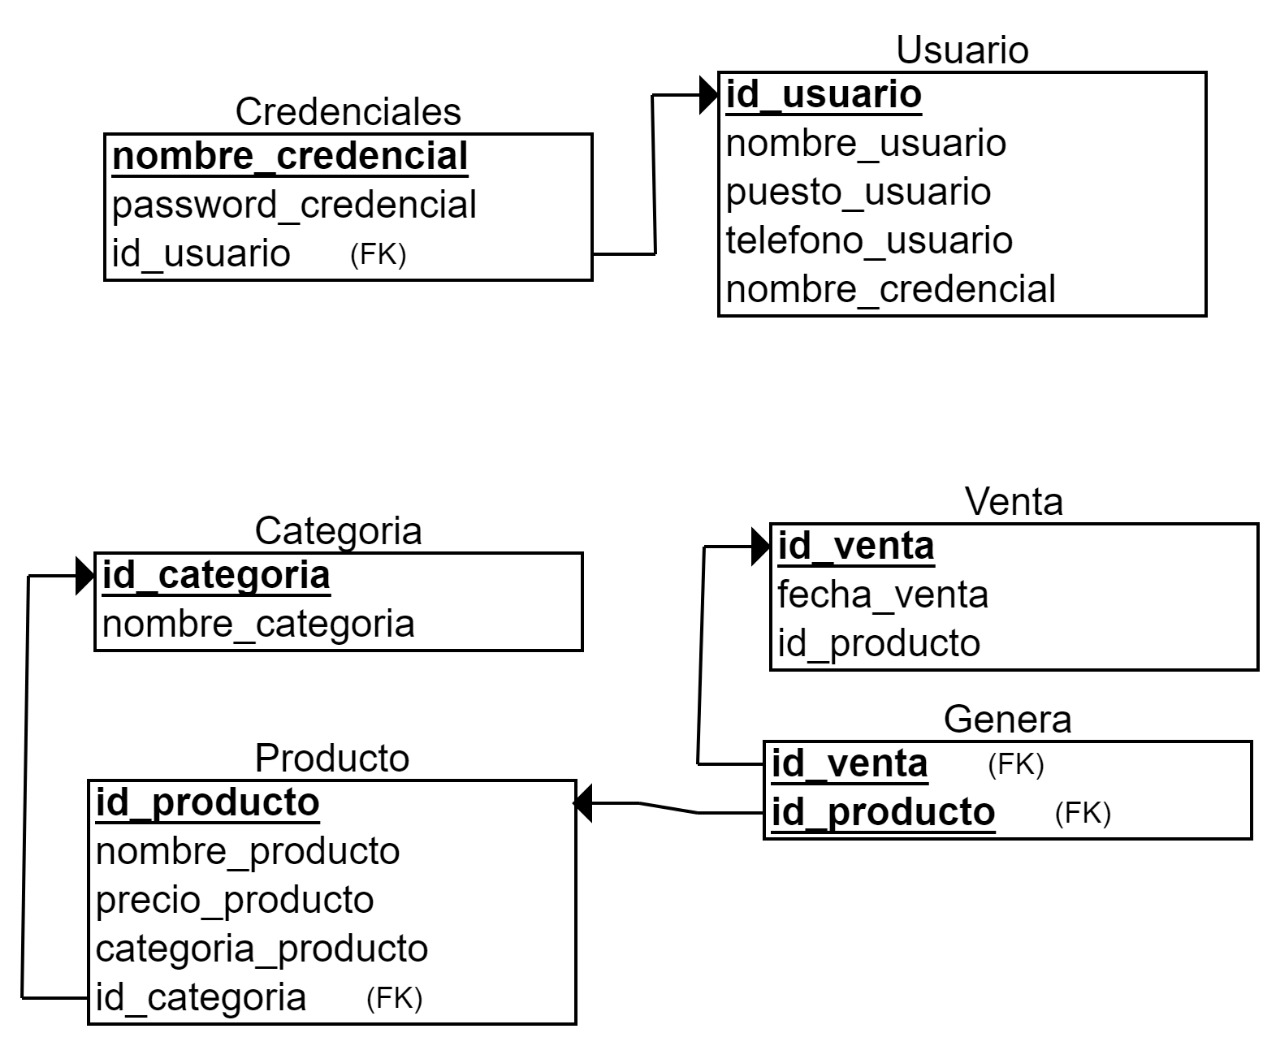
\includegraphics[scale=.45]{modeloRelacional}
		\centering
		\caption{Diagrama General de base de datos}
		\label{img:modeloRelacional}
	\end{figure} 

\pagebreak

\subsection{
	\textit{
		\color{colorESCOM}{Diccionario de datos}
	}
}

En la presente sección se describen las diversas tablas con sus respectivas columnas

\begin{itemize}
	\item \textbf{Tabla:} Credencial
			\begin{figure}[H]
				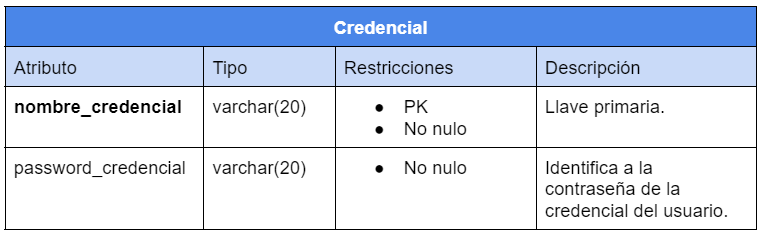
\includegraphics[scale=.54]{tablaCredencial}
				\centering
				\label{img:tablaCredencial}
			\end{figure} 
			
	\item \textbf{Tabla:} Usuario
			\begin{figure}[H]
				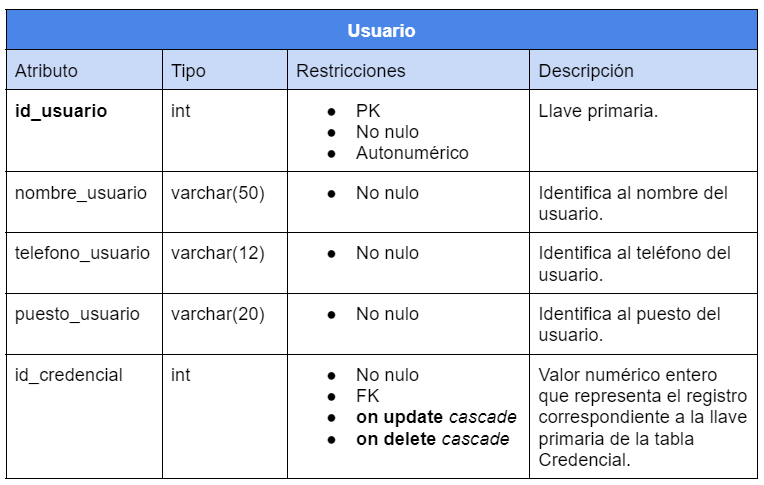
\includegraphics[scale=.54]{tablaUsuario}
				\centering
				\label{img:tablaUsuario}
			\end{figure} 
			
	\item \textbf{Tabla:} Categoria
			\begin{figure}[H]
				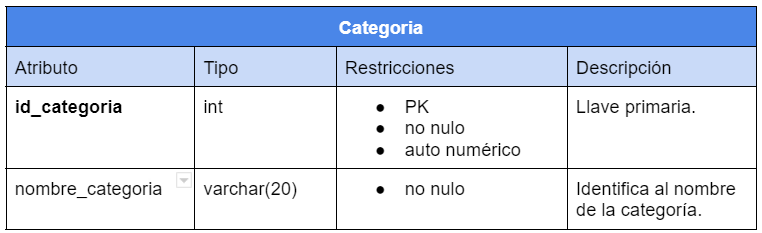
\includegraphics[scale=.54]{tablaCategoria}
				\centering
				\label{img:tablaCategoria}
			\end{figure} 

\pagebreak

	\item \textbf{Tabla:} Producto
			\begin{figure}[H]
				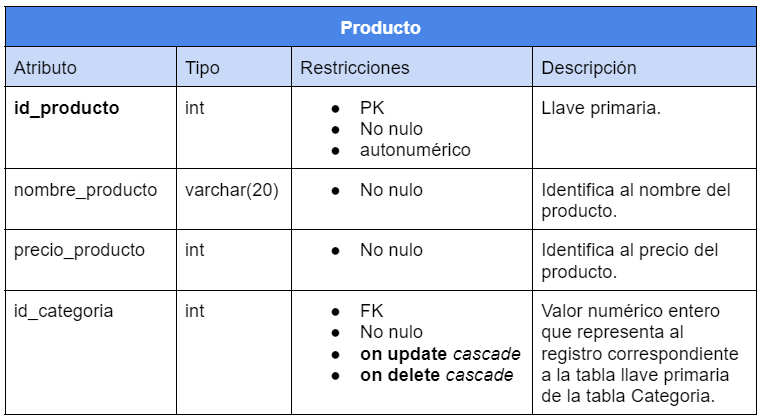
\includegraphics[scale=.54]{tablaProducto}
				\centering
				\label{img:tablaProducto}
			\end{figure} 
			
	\item \textbf{Tabla:} Venta
			\begin{figure}[H]
				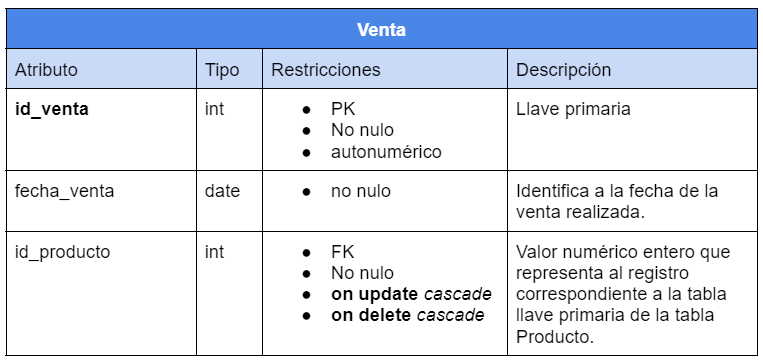
\includegraphics[scale=.54]{tablaVenta}
				\centering
				\label{img:tablaVenta}
			\end{figure} 
\end{itemize}

\pagebreak

%################################################
\section{\color{colorIPN}{Conclusión}}
El proyecto tiene intención de mejorar la administración y manejo de cualquier tienda de conveniencia, mediante el uso de una página web enlazada con la base de datos presentada en este documento. 

Se considera que los modelos realizado satisfacen correctamente las necesidades del cliente y el diccionario de datos establece explícitamente las características de cada tabla y columna.

\color{colorIPN}{
	\begin{flushright}
		\textit{
			Aguirre\\
			Hernández\\			
			Hurtado Morales Emiliano\\
			Martínez
		}
	\end{flushright} \hfill \break
}

\pagebreak

%################################################

\section{\color{colorIPN}{Referencias Bibliográficas}}
\color{colorESCOM}{
	\begin{thebibliography}{10}
		\bibitem[ESCOM-IPN, 2022]{ESCOM-IPN}
		Enríquez, J	.
		\newblock {\em Eventos Web. Base de Datos y Diccionario de Datos de Eventos Web.}
		\newblock Recuperado el 17 de marzo de 2022, de https://tinyurl.com/bp97axx8
	
		\bibitem[Economipedia, 2022]{Economipedia}
		Rus, E.
		\newblock {\em Modelo Relacional.}
		\newblock Recuperado el 17 de marzo de 2022, de https://tinyurl.com/2p8ftrvx
	
		\bibitem[UMH, 2022]{UMH}
		UMH.
		\newblock {\em El Modelo de Datos Entidad-Relación.}
		\newblock Recuperado el 17 de marzo de 2022, de https://tinyurl.com/ppyf3cmt
		
		\bibitem[SEDIA, 2021]{SEDIA}
		SEDIA
		\newblock {\em ¿Qué es un diccionario de datos y por qué es importante?}
		\newblock Recuperado el 17 de marzo de 2022, de https://datos.gob.es/es/blog/que-es-un-diccionario-de-datos-y-por-que-es-importante
	\end{thebibliography}
}

\end{document}
